\documentclass[14pt]{extbook}
\usepackage{multicol, enumerate, enumitem, hyperref, color, soul, setspace, parskip, fancyhdr} %General Packages
\usepackage{amssymb, amsthm, amsmath, latexsym, units, mathtools} %Math Packages
\everymath{\displaystyle} %All math in Display Style
% Packages with additional options
\usepackage[headsep=0.5cm,headheight=12pt, left=1 in,right= 1 in,top= 1 in,bottom= 1 in]{geometry}
\usepackage[usenames,dvipsnames]{xcolor}
\usepackage{dashrule}  % Package to use the command below to create lines between items
\newcommand{\litem}[1]{\item#1\hspace*{-1cm}\rule{\textwidth}{0.4pt}}
\pagestyle{fancy}
\lhead{Progress Quiz 9}
\chead{}
\rhead{Version ALL}
\lfoot{9541-5764}
\cfoot{}
\rfoot{Summer C 2021}
\begin{document}

\begin{enumerate}
\litem{
Construct the lowest-degree polynomial given the zeros below. Then, choose the intervals that contain the coefficients of the polynomial in the form $ax^3+bx^2+cx+d$.\[ \frac{-3}{4}, \frac{7}{4}, \text{ and } \frac{1}{5} \]\begin{enumerate}[label=\Alph*.]
\item \( a \in [71, 88], b \in [-99, -95], c \in [-89, -81], \text{ and } d \in [-25, -15] \)
\item \( a \in [71, 88], b \in [-222, -215], c \in [143, 147], \text{ and } d \in [-25, -15] \)
\item \( a \in [71, 88], b \in [-99, -95], c \in [-89, -81], \text{ and } d \in [16, 31] \)
\item \( a \in [71, 88], b \in [57, 67], c \in [-121, -119], \text{ and } d \in [16, 31] \)
\item \( a \in [71, 88], b \in [94, 102], c \in [-89, -81], \text{ and } d \in [-25, -15] \)

\end{enumerate} }
\litem{
Describe the end behavior of the polynomial below.\[ f(x) = 7(x - 7)^{4}(x + 7)^{7}(x - 3)^{2}(x + 3)^{2} \]\begin{enumerate}[label=\Alph*.]
\begin{multicols}{2}\item 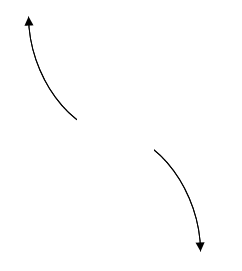
\includegraphics[width = 0.3\textwidth]{../Figures/polyEndBehaviorCopyAA.png}\item 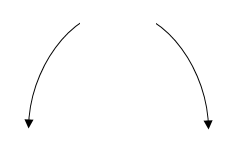
\includegraphics[width = 0.3\textwidth]{../Figures/polyEndBehaviorCopyBA.png}\item 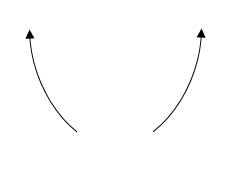
\includegraphics[width = 0.3\textwidth]{../Figures/polyEndBehaviorCopyCA.png}\item 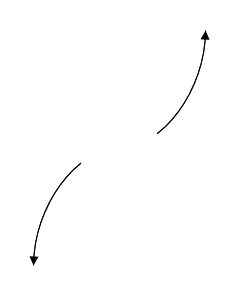
\includegraphics[width = 0.3\textwidth]{../Figures/polyEndBehaviorCopyDA.png}\end{multicols}\item None of the above.
\end{enumerate} }
\litem{
Construct the lowest-degree polynomial given the zeros below. Then, choose the intervals that contain the coefficients of the polynomial in the form $x^3+bx^2+cx+d$.\[ 5 - 4 i \text{ and } -4 \]\begin{enumerate}[label=\Alph*.]
\item \( b \in [3, 20], c \in [-0.68, 1.9], \text{ and } d \in [-168, -161] \)
\item \( b \in [-1, 4], c \in [5.04, 8.21], \text{ and } d \in [16, 23] \)
\item \( b \in [-6, -4], c \in [-0.68, 1.9], \text{ and } d \in [164, 166] \)
\item \( b \in [-1, 4], c \in [-1.45, 0.42], \text{ and } d \in [-20, -17] \)
\item \( \text{None of the above.} \)

\end{enumerate} }
\litem{
Which of the following equations \textit{could} be of the graph presented below?
\begin{center}
    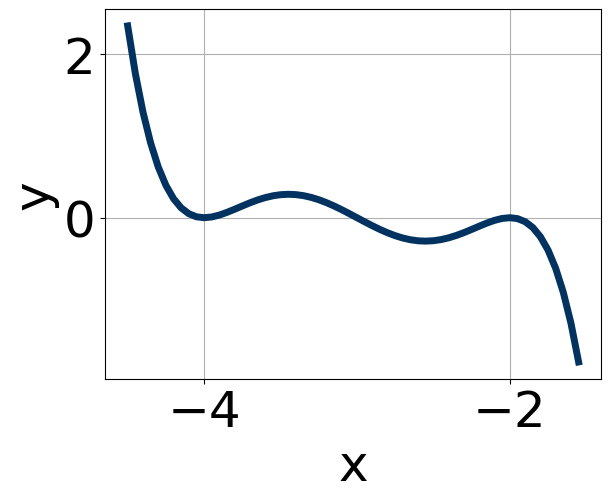
\includegraphics[width=0.5\textwidth]{../Figures/polyGraphToFunctionCopyA.png}
\end{center}
\begin{enumerate}[label=\Alph*.]
\item \( -13(x + 2)^{10} (x + 4)^{7} (x + 3)^{6} \)
\item \( 18(x + 2)^{10} (x + 4)^{6} (x + 3)^{10} \)
\item \( 16(x + 2)^{4} (x + 4)^{4} (x + 3)^{5} \)
\item \( -6(x + 2)^{10} (x + 4)^{6} (x + 3)^{5} \)
\item \( -15(x + 2)^{6} (x + 4)^{7} (x + 3)^{11} \)

\end{enumerate} }
\litem{
Describe the zero behavior of the zero $x = -8$ of the polynomial below.\[ f(x) = 6(x + 7)^{3}(x - 7)^{2}(x - 8)^{5}(x + 8)^{4} \]\begin{enumerate}[label=\Alph*.]
\begin{multicols}{2}\item 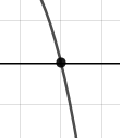
\includegraphics[width = 0.3\textwidth]{../Figures/polyZeroBehaviorCopyAA.png}\item 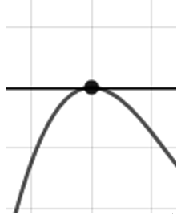
\includegraphics[width = 0.3\textwidth]{../Figures/polyZeroBehaviorCopyBA.png}\item 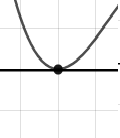
\includegraphics[width = 0.3\textwidth]{../Figures/polyZeroBehaviorCopyCA.png}\item 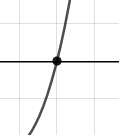
\includegraphics[width = 0.3\textwidth]{../Figures/polyZeroBehaviorCopyDA.png}\end{multicols}\item None of the above.
\end{enumerate} }
\litem{
Describe the zero behavior of the zero $x = -9$ of the polynomial below.\[ f(x) = -2(x + 9)^{6}(x - 9)^{9}(x - 8)^{2}(x + 8)^{5} \]\begin{enumerate}[label=\Alph*.]
\begin{multicols}{2}\item 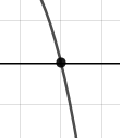
\includegraphics[width = 0.3\textwidth]{../Figures/polyZeroBehaviorAA.png}\item 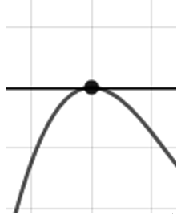
\includegraphics[width = 0.3\textwidth]{../Figures/polyZeroBehaviorBA.png}\item 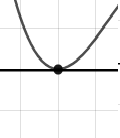
\includegraphics[width = 0.3\textwidth]{../Figures/polyZeroBehaviorCA.png}\item 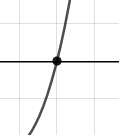
\includegraphics[width = 0.3\textwidth]{../Figures/polyZeroBehaviorDA.png}\end{multicols}\item None of the above.
\end{enumerate} }
\litem{
Describe the end behavior of the polynomial below.\[ f(x) = -4(x - 2)^{3}(x + 2)^{4}(x - 9)^{5}(x + 9)^{5} \]\begin{enumerate}[label=\Alph*.]
\begin{multicols}{2}\item 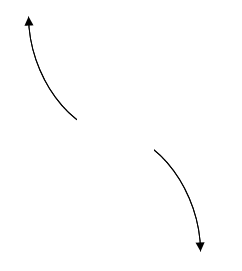
\includegraphics[width = 0.3\textwidth]{../Figures/polyEndBehaviorAA.png}\item 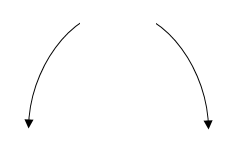
\includegraphics[width = 0.3\textwidth]{../Figures/polyEndBehaviorBA.png}\item 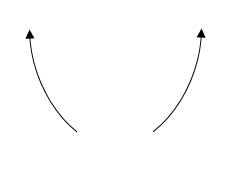
\includegraphics[width = 0.3\textwidth]{../Figures/polyEndBehaviorCA.png}\item 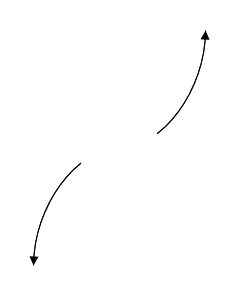
\includegraphics[width = 0.3\textwidth]{../Figures/polyEndBehaviorDA.png}\end{multicols}\item None of the above.
\end{enumerate} }
\litem{
Construct the lowest-degree polynomial given the zeros below. Then, choose the intervals that contain the coefficients of the polynomial in the form $x^3+bx^2+cx+d$.\[ -3 + 2 i \text{ and } 1 \]\begin{enumerate}[label=\Alph*.]
\item \( b \in [-6.2, -2.7], c \in [7, 14], \text{ and } d \in [10, 14] \)
\item \( b \in [1.3, 5.6], c \in [7, 14], \text{ and } d \in [-16, -7] \)
\item \( b \in [-0.3, 3.3], c \in [-2, 3], \text{ and } d \in [-5, 0] \)
\item \( b \in [-0.3, 3.3], c \in [-6, -1], \text{ and } d \in [0, 3] \)
\item \( \text{None of the above.} \)

\end{enumerate} }
\litem{
Construct the lowest-degree polynomial given the zeros below. Then, choose the intervals that contain the coefficients of the polynomial in the form $ax^3+bx^2+cx+d$.\[ \frac{-5}{4}, \frac{-3}{4}, \text{ and } 5 \]\begin{enumerate}[label=\Alph*.]
\item \( a \in [15, 19], b \in [42, 52], c \in [-151, -140], \text{ and } d \in [68, 80] \)
\item \( a \in [15, 19], b \in [-48, -41], c \in [-151, -140], \text{ and } d \in [68, 80] \)
\item \( a \in [15, 19], b \in [-48, -41], c \in [-151, -140], \text{ and } d \in [-76, -69] \)
\item \( a \in [15, 19], b \in [-94, -79], c \in [23, 34], \text{ and } d \in [68, 80] \)
\item \( a \in [15, 19], b \in [-119, -111], c \in [173, 179], \text{ and } d \in [-76, -69] \)

\end{enumerate} }
\litem{
Which of the following equations \textit{could} be of the graph presented below?
\begin{center}
    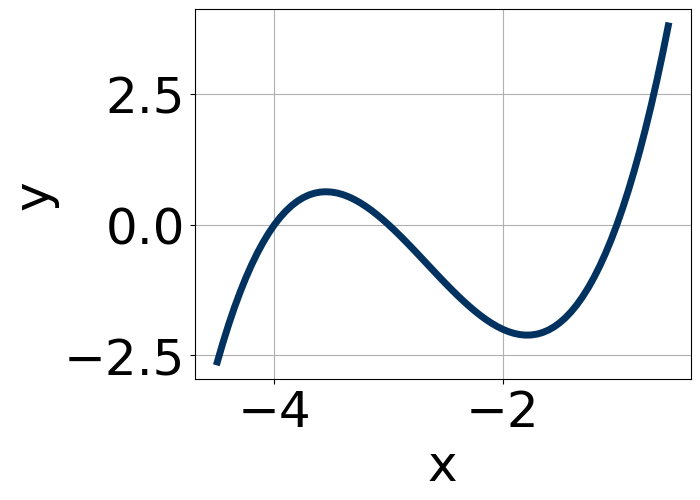
\includegraphics[width=0.5\textwidth]{../Figures/polyGraphToFunctionA.png}
\end{center}
\begin{enumerate}[label=\Alph*.]
\item \( 5(x + 1)^{8} (x + 3)^{4} (x + 4)^{5} \)
\item \( -17(x + 1)^{4} (x + 3)^{5} (x + 4)^{5} \)
\item \( 10(x + 1)^{11} (x + 3)^{7} (x + 4)^{11} \)
\item \( 5(x + 1)^{4} (x + 3)^{11} (x + 4)^{11} \)
\item \( -9(x + 1)^{7} (x + 3)^{11} (x + 4)^{9} \)

\end{enumerate} }
\litem{
Construct the lowest-degree polynomial given the zeros below. Then, choose the intervals that contain the coefficients of the polynomial in the form $ax^3+bx^2+cx+d$.\[ \frac{5}{2}, \frac{-1}{2}, \text{ and } -7 \]\begin{enumerate}[label=\Alph*.]
\item \( a \in [2, 10], b \in [36.1, 42.5], c \in [86, 95], \text{ and } d \in [30, 40] \)
\item \( a \in [2, 10], b \in [18.8, 21.8], c \in [-65, -58], \text{ and } d \in [-35, -32] \)
\item \( a \in [2, 10], b \in [35.9, 37.2], c \in [42, 60], \text{ and } d \in [-35, -32] \)
\item \( a \in [2, 10], b \in [-22.7, -19.9], c \in [-65, -58], \text{ and } d \in [30, 40] \)
\item \( a \in [2, 10], b \in [18.8, 21.8], c \in [-65, -58], \text{ and } d \in [30, 40] \)

\end{enumerate} }
\litem{
Describe the end behavior of the polynomial below.\[ f(x) = -6(x - 6)^{3}(x + 6)^{6}(x + 2)^{3}(x - 2)^{3} \]\begin{enumerate}[label=\Alph*.]
\begin{multicols}{2}\item 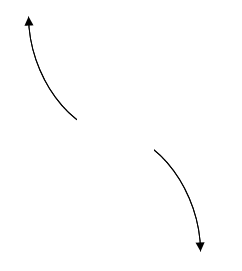
\includegraphics[width = 0.3\textwidth]{../Figures/polyEndBehaviorCopyAB.png}\item 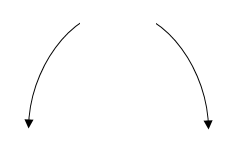
\includegraphics[width = 0.3\textwidth]{../Figures/polyEndBehaviorCopyBB.png}\item 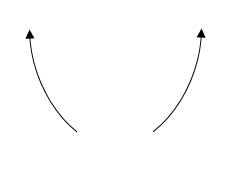
\includegraphics[width = 0.3\textwidth]{../Figures/polyEndBehaviorCopyCB.png}\item 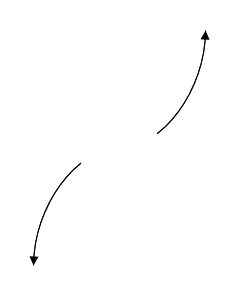
\includegraphics[width = 0.3\textwidth]{../Figures/polyEndBehaviorCopyDB.png}\end{multicols}\item None of the above.
\end{enumerate} }
\litem{
Construct the lowest-degree polynomial given the zeros below. Then, choose the intervals that contain the coefficients of the polynomial in the form $x^3+bx^2+cx+d$.\[ 4 - 3 i \text{ and } 2 \]\begin{enumerate}[label=\Alph*.]
\item \( b \in [-15, -8], c \in [35, 44], \text{ and } d \in [-50, -44] \)
\item \( b \in [-5, 4], c \in [1, 7], \text{ and } d \in [-8, 2] \)
\item \( b \in [10, 15], c \in [35, 44], \text{ and } d \in [50, 56] \)
\item \( b \in [-5, 4], c \in [-9, 0], \text{ and } d \in [6, 11] \)
\item \( \text{None of the above.} \)

\end{enumerate} }
\litem{
Which of the following equations \textit{could} be of the graph presented below?
\begin{center}
    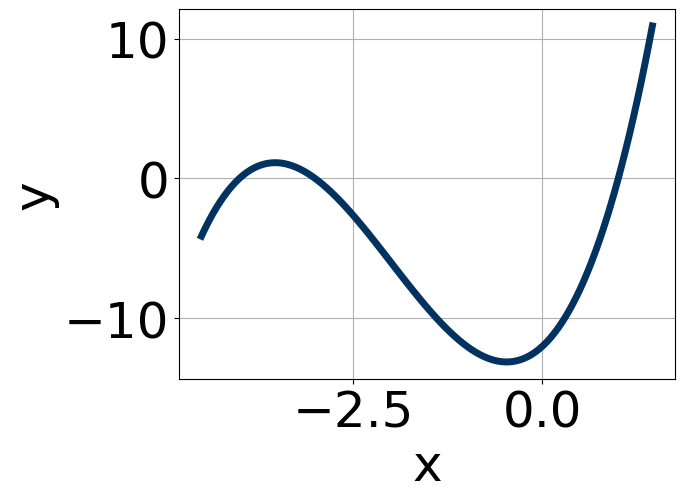
\includegraphics[width=0.5\textwidth]{../Figures/polyGraphToFunctionCopyB.png}
\end{center}
\begin{enumerate}[label=\Alph*.]
\item \( 15(x - 1)^{4} (x + 3)^{4} (x + 4)^{9} \)
\item \( -12(x - 1)^{10} (x + 3)^{11} (x + 4)^{11} \)
\item \( -11(x - 1)^{11} (x + 3)^{7} (x + 4)^{7} \)
\item \( 3(x - 1)^{7} (x + 3)^{9} (x + 4)^{9} \)
\item \( 20(x - 1)^{8} (x + 3)^{5} (x + 4)^{9} \)

\end{enumerate} }
\litem{
Describe the zero behavior of the zero $x = 4$ of the polynomial below.\[ f(x) = -6(x - 4)^{2}(x + 4)^{3}(x - 8)^{2}(x + 8)^{5} \]\begin{enumerate}[label=\Alph*.]
\begin{multicols}{2}\item 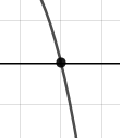
\includegraphics[width = 0.3\textwidth]{../Figures/polyZeroBehaviorCopyAB.png}\item 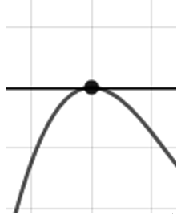
\includegraphics[width = 0.3\textwidth]{../Figures/polyZeroBehaviorCopyBB.png}\item 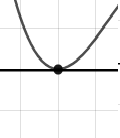
\includegraphics[width = 0.3\textwidth]{../Figures/polyZeroBehaviorCopyCB.png}\item 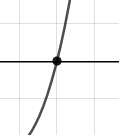
\includegraphics[width = 0.3\textwidth]{../Figures/polyZeroBehaviorCopyDB.png}\end{multicols}\item None of the above.
\end{enumerate} }
\litem{
Describe the zero behavior of the zero $x = 5$ of the polynomial below.\[ f(x) = -5(x + 5)^{3}(x - 5)^{4}(x + 7)^{2}(x - 7)^{4} \]\begin{enumerate}[label=\Alph*.]
\begin{multicols}{2}\item 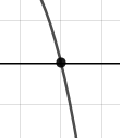
\includegraphics[width = 0.3\textwidth]{../Figures/polyZeroBehaviorAB.png}\item 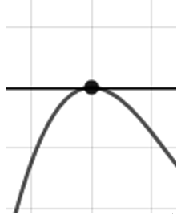
\includegraphics[width = 0.3\textwidth]{../Figures/polyZeroBehaviorBB.png}\item 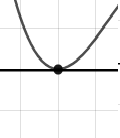
\includegraphics[width = 0.3\textwidth]{../Figures/polyZeroBehaviorCB.png}\item 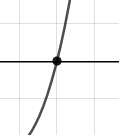
\includegraphics[width = 0.3\textwidth]{../Figures/polyZeroBehaviorDB.png}\end{multicols}\item None of the above.
\end{enumerate} }
\litem{
Describe the end behavior of the polynomial below.\[ f(x) = 6(x - 6)^{4}(x + 6)^{7}(x - 5)^{3}(x + 5)^{4} \]\begin{enumerate}[label=\Alph*.]
\begin{multicols}{2}\item 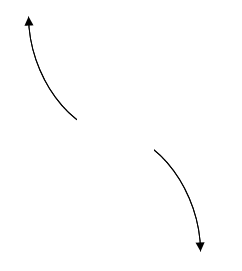
\includegraphics[width = 0.3\textwidth]{../Figures/polyEndBehaviorAB.png}\item 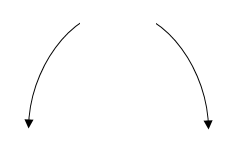
\includegraphics[width = 0.3\textwidth]{../Figures/polyEndBehaviorBB.png}\item 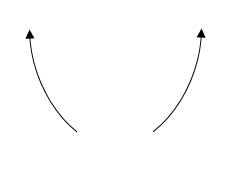
\includegraphics[width = 0.3\textwidth]{../Figures/polyEndBehaviorCB.png}\item 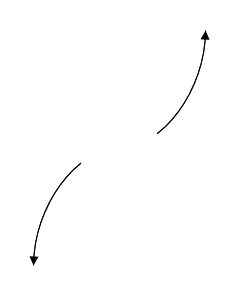
\includegraphics[width = 0.3\textwidth]{../Figures/polyEndBehaviorDB.png}\end{multicols}\item None of the above.
\end{enumerate} }
\litem{
Construct the lowest-degree polynomial given the zeros below. Then, choose the intervals that contain the coefficients of the polynomial in the form $x^3+bx^2+cx+d$.\[ -3 - 4 i \text{ and } 1 \]\begin{enumerate}[label=\Alph*.]
\item \( b \in [-2.7, 4.7], c \in [0.81, 2.83], \text{ and } d \in [-3.5, -2.56] \)
\item \( b \in [-7.9, -3.5], c \in [17.28, 19.46], \text{ and } d \in [24.68, 25.62] \)
\item \( b \in [-2.7, 4.7], c \in [2.24, 5.06], \text{ and } d \in [-4.56, -3.05] \)
\item \( b \in [3.6, 7.4], c \in [17.28, 19.46], \text{ and } d \in [-25.02, -24.7] \)
\item \( \text{None of the above.} \)

\end{enumerate} }
\litem{
Construct the lowest-degree polynomial given the zeros below. Then, choose the intervals that contain the coefficients of the polynomial in the form $ax^3+bx^2+cx+d$.\[ \frac{-2}{3}, \frac{1}{3}, \text{ and } \frac{5}{4} \]\begin{enumerate}[label=\Alph*.]
\item \( a \in [35, 37], b \in [-38, -31], c \in [-31, -22], \text{ and } d \in [-13, -7] \)
\item \( a \in [35, 37], b \in [-38, -31], c \in [-31, -22], \text{ and } d \in [8, 17] \)
\item \( a \in [35, 37], b \in [-60, -55], c \in [4, 16], \text{ and } d \in [8, 17] \)
\item \( a \in [35, 37], b \in [-86, -76], c \in [53, 57], \text{ and } d \in [-13, -7] \)
\item \( a \in [35, 37], b \in [32, 39], c \in [-31, -22], \text{ and } d \in [-13, -7] \)

\end{enumerate} }
\litem{
Which of the following equations \textit{could} be of the graph presented below?
\begin{center}
    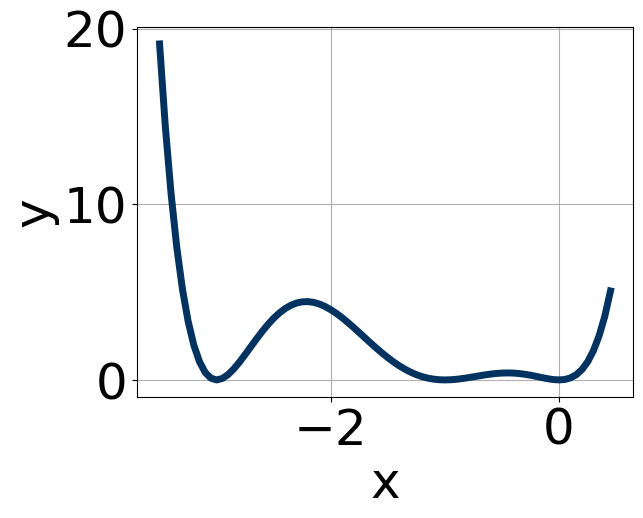
\includegraphics[width=0.5\textwidth]{../Figures/polyGraphToFunctionB.png}
\end{center}
\begin{enumerate}[label=\Alph*.]
\item \( 4x^{10} (x + 3)^{10} (x + 1)^{6} \)
\item \( 10x^{8} (x + 3)^{8} (x + 1)^{11} \)
\item \( 6x^{5} (x + 3)^{4} (x + 1)^{9} \)
\item \( -15x^{10} (x + 3)^{4} (x + 1)^{10} \)
\item \( -6x^{6} (x + 3)^{8} (x + 1)^{5} \)

\end{enumerate} }
\litem{
Construct the lowest-degree polynomial given the zeros below. Then, choose the intervals that contain the coefficients of the polynomial in the form $ax^3+bx^2+cx+d$.\[ \frac{4}{3}, \frac{2}{3}, \text{ and } \frac{3}{5} \]\begin{enumerate}[label=\Alph*.]
\item \( a \in [43, 49], b \in [-121, -109], c \in [94, 102], \text{ and } d \in [-30, -23] \)
\item \( a \in [43, 49], b \in [115, 126], c \in [94, 102], \text{ and } d \in [24, 25] \)
\item \( a \in [43, 49], b \in [2, 5], c \in [-61, -52], \text{ and } d \in [24, 25] \)
\item \( a \in [43, 49], b \in [63, 65], c \in [-21, -6], \text{ and } d \in [-30, -23] \)
\item \( a \in [43, 49], b \in [-121, -109], c \in [94, 102], \text{ and } d \in [24, 25] \)

\end{enumerate} }
\litem{
Describe the end behavior of the polynomial below.\[ f(x) = 8(x - 9)^{5}(x + 9)^{10}(x - 3)^{3}(x + 3)^{5} \]\begin{enumerate}[label=\Alph*.]
\begin{multicols}{2}\item 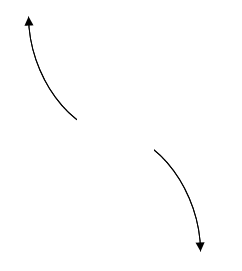
\includegraphics[width = 0.3\textwidth]{../Figures/polyEndBehaviorCopyAC.png}\item 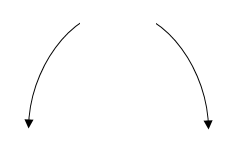
\includegraphics[width = 0.3\textwidth]{../Figures/polyEndBehaviorCopyBC.png}\item 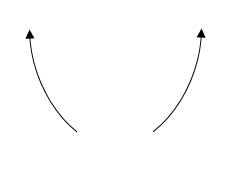
\includegraphics[width = 0.3\textwidth]{../Figures/polyEndBehaviorCopyCC.png}\item 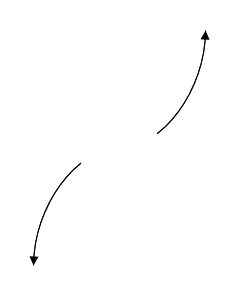
\includegraphics[width = 0.3\textwidth]{../Figures/polyEndBehaviorCopyDC.png}\end{multicols}\item None of the above.
\end{enumerate} }
\litem{
Construct the lowest-degree polynomial given the zeros below. Then, choose the intervals that contain the coefficients of the polynomial in the form $x^3+bx^2+cx+d$.\[ 2 + 4 i \text{ and } 1 \]\begin{enumerate}[label=\Alph*.]
\item \( b \in [4.8, 7.3], c \in [22.72, 24.73], \text{ and } d \in [18.8, 23.2] \)
\item \( b \in [-0.5, 1.6], c \in [-4.03, -2.68], \text{ and } d \in [0.5, 2.3] \)
\item \( b \in [-8.6, -2.1], c \in [22.72, 24.73], \text{ and } d \in [-21.3, -19.8] \)
\item \( b \in [-0.5, 1.6], c \in [-5.22, -3.99], \text{ and } d \in [2.7, 7] \)
\item \( \text{None of the above.} \)

\end{enumerate} }
\litem{
Which of the following equations \textit{could} be of the graph presented below?
\begin{center}
    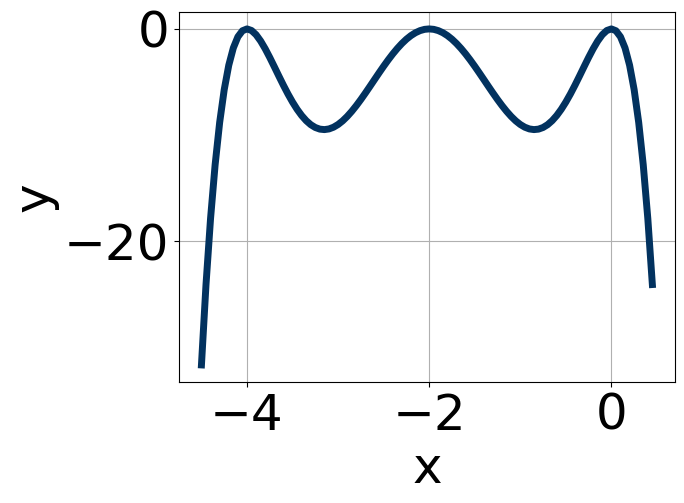
\includegraphics[width=0.5\textwidth]{../Figures/polyGraphToFunctionCopyC.png}
\end{center}
\begin{enumerate}[label=\Alph*.]
\item \( 18x^{5} (x + 2)^{8} (x + 4)^{4} \)
\item \( 9x^{10} (x + 2)^{8} (x + 4)^{6} \)
\item \( -6x^{5} (x + 2)^{8} (x + 4)^{6} \)
\item \( -3x^{4} (x + 2)^{8} (x + 4)^{8} \)
\item \( -14x^{5} (x + 2)^{6} (x + 4)^{5} \)

\end{enumerate} }
\litem{
Describe the zero behavior of the zero $x = 9$ of the polynomial below.\[ f(x) = 9(x - 3)^{11}(x + 3)^{8}(x - 9)^{10}(x + 9)^{9} \]\begin{enumerate}[label=\Alph*.]
\begin{multicols}{2}\item 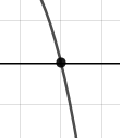
\includegraphics[width = 0.3\textwidth]{../Figures/polyZeroBehaviorCopyAC.png}\item 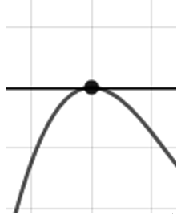
\includegraphics[width = 0.3\textwidth]{../Figures/polyZeroBehaviorCopyBC.png}\item 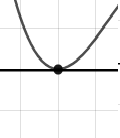
\includegraphics[width = 0.3\textwidth]{../Figures/polyZeroBehaviorCopyCC.png}\item 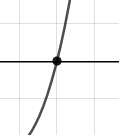
\includegraphics[width = 0.3\textwidth]{../Figures/polyZeroBehaviorCopyDC.png}\end{multicols}\item None of the above.
\end{enumerate} }
\litem{
Describe the zero behavior of the zero $x = 4$ of the polynomial below.\[ f(x) = 5(x + 6)^{5}(x - 6)^{4}(x + 4)^{9}(x - 4)^{6} \]\begin{enumerate}[label=\Alph*.]
\begin{multicols}{2}\item 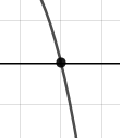
\includegraphics[width = 0.3\textwidth]{../Figures/polyZeroBehaviorAC.png}\item 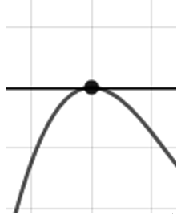
\includegraphics[width = 0.3\textwidth]{../Figures/polyZeroBehaviorBC.png}\item 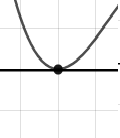
\includegraphics[width = 0.3\textwidth]{../Figures/polyZeroBehaviorCC.png}\item 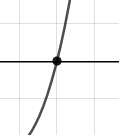
\includegraphics[width = 0.3\textwidth]{../Figures/polyZeroBehaviorDC.png}\end{multicols}\item None of the above.
\end{enumerate} }
\litem{
Describe the end behavior of the polynomial below.\[ f(x) = 2(x + 4)^{3}(x - 4)^{8}(x - 5)^{5}(x + 5)^{6} \]\begin{enumerate}[label=\Alph*.]
\begin{multicols}{2}\item 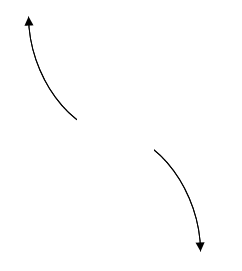
\includegraphics[width = 0.3\textwidth]{../Figures/polyEndBehaviorAC.png}\item \includegraphics[width = 0.3\textwidth]{../Figures/polyEndBehaviorBC.png}\item \includegraphics[width = 0.3\textwidth]{../Figures/polyEndBehaviorCC.png}\item \includegraphics[width = 0.3\textwidth]{../Figures/polyEndBehaviorDC.png}\end{multicols}\item None of the above.
\end{enumerate} }
\litem{
Construct the lowest-degree polynomial given the zeros below. Then, choose the intervals that contain the coefficients of the polynomial in the form $x^3+bx^2+cx+d$.\[ -4 - 3 i \text{ and } 1 \]\begin{enumerate}[label=\Alph*.]
\item \( b \in [-2.3, 1.9], c \in [1.81, 2.56], \text{ and } d \in [-3.42, -2.96] \)
\item \( b \in [-8.3, -5.2], c \in [15.94, 17.54], \text{ and } d \in [24.44, 26.01] \)
\item \( b \in [4.9, 8.8], c \in [15.94, 17.54], \text{ and } d \in [-26.86, -23.36] \)
\item \( b \in [-2.3, 1.9], c \in [2.49, 3.29], \text{ and } d \in [-4.03, -3.82] \)
\item \( \text{None of the above.} \)

\end{enumerate} }
\litem{
Construct the lowest-degree polynomial given the zeros below. Then, choose the intervals that contain the coefficients of the polynomial in the form $ax^3+bx^2+cx+d$.\[ \frac{-7}{4}, \frac{7}{2}, \text{ and } \frac{-3}{5} \]\begin{enumerate}[label=\Alph*.]
\item \( a \in [33, 45], b \in [-46, -44], c \in [-295, -277], \text{ and } d \in [-147, -143] \)
\item \( a \in [33, 45], b \in [90, 98], c \in [-205, -195], \text{ and } d \in [-147, -143] \)
\item \( a \in [33, 45], b \in [35, 50], c \in [-295, -277], \text{ and } d \in [146, 151] \)
\item \( a \in [33, 45], b \in [-186, -184], c \in [111, 127], \text{ and } d \in [146, 151] \)
\item \( a \in [33, 45], b \in [-46, -44], c \in [-295, -277], \text{ and } d \in [146, 151] \)

\end{enumerate} }
\litem{
Which of the following equations \textit{could} be of the graph presented below?
\begin{center}
    \includegraphics[width=0.5\textwidth]{../Figures/polyGraphToFunctionC.png}
\end{center}
\begin{enumerate}[label=\Alph*.]
\item \( 6x^{9} (x - 1)^{4} (x - 3)^{5} \)
\item \( 19x^{11} (x - 1)^{8} (x - 3)^{6} \)
\item \( 9x^{4} (x - 1)^{10} (x - 3)^{9} \)
\item \( -8x^{10} (x - 1)^{8} (x - 3)^{7} \)
\item \( -11x^{4} (x - 1)^{8} (x - 3)^{8} \)

\end{enumerate} }
\end{enumerate}

\end{document}